\section{Wiktor Deka}
\label{sec:Wiktor Deka}

\subsection{Wyrażenia matematyczne}
\textbf{Wzór na deltę: }
\begin{equation}
    \Delta = b^2 - 4ac 
\end{equation}

\noindent \textbf{A na pierwiastki kwadratowe:}
\begin{equation}
x = \frac{-b \pm \Delta}{2a}
\end{equation}

\noindent\textbf{Małe twierdzenie Fermata: }

\begin{quote}
    \begin{center}
        Jeżeli a $\in Z, p \in P$ to $a^p$ =  a(mod p)
    \end{center}
\end{quote}


\subsection{Zdjęcie}
\begin{figure}[htbp]
    \centering
    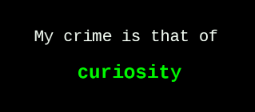
\includegraphics[width=0.6\textwidth]{pictures/crime.png}
    \caption{Przerażający postulat przerażających hakerów z przerażającego filmu z 1995}
    \label{fig:curiosity}
\end{figure}

Obrazek ~\ref{fig:curiosity} ustawiłem sobie nawet na tapetę

\subsection{Tabela}
\begin{center}
    \begin{tabular}{c|c|c}
      O & X & X \\      \hline
      X & O & X \\      \hline
      X & X & O
    \label{tab:tic_tac_toe}
    \end{tabular}
\end{center}

Tabela~\ref{tab:tic_tac_toe} pokazuje znaną grę kółko i krzyżyk

\subsection{Lista numerowana i nienumerowana}

\begin{enumerate}
    \item Pytanie 1
    \begin{enumerate}
        \item odp1
        \item odp2
        \item odp3
        \item odp4
    \end{enumerate}
    \item Pytanie 2
    \begin{enumerate}
        \item Być albo nie być
        \begin{enumerate}
            \item Oto jest pytanie?
            \item być
            \begin{description}
                \item Być albo nie być, ty jesteś jak zdrowie.
                \item Ile cię cenić trzeba, ten tylko się dowie,
                \item gdy Hamlet, książę duński przyjedzie na krowie.
            \end{description}
            \item nie być
            \begin{enumerate}
                \item \item Oto jest pytanie
            \end{enumerate}
        \end{enumerate}
    \end{enumerate}
\end{enumerate}

\subsection{Inwokacja}

Litwo, Ojczyzno moja! ty jesteś jak zdrowie;
Ile cię trzeba cenić, ten tylko się dowie,
Kto cię stracił. Dziś piękność twą w całej ozdobie
Widzę i opisuję, bo tęsknię po tobie.

\textbf{\textit{Tymczasem, przenoś moją duszę utęsknioną
Do tych pagórków leśnych, do tych łąk zielonych,}}
Panno święta, co Jasnej bronisz Częstochowy
I w Ostrej świecisz Bramie! Ty, co gród zamkowy
Nowogródzki ochraniasz z jego wiernym ludem!
Jak mnie dziecko do zdrowia powróciłaś cudem
(— Gdy od płaczącej matki, pod Twoją opiekę
Ofiarowany martwą podniosłem powiekę;
I zaraz mogłem pieszo, do Twych świątyń progu
Iść za wrócone życie podziękować Bogu —)
Tak nas powrócisz cudem na Ojczyzny łono!...

\underline{\textbf{Szeroko nad błękitnym Niemnem rozciągnionych;}}
Do tych pól malowanych zbożem rozmaitem,
Wyzłacanych pszenicą, posrebrzanych żytem;
Gdzie bursztynowy świerzop, gryka jak śnieg biała
Gdzie panieńskim rumieńcem dzięcielina pała,
A wszystko przepasane jakby wstęgą, miedzą
Zieloną, na niej zrzadka ciche grusze siedzą.
